\documentclass[12pt,pdf,hyperref={unicode}]{beamer}
\beamertemplatenavigationsymbolsempty
\setbeamertemplate{footline}[page number]
\usepackage[utf8]{inputenc}
\usepackage{bm}
\usepackage{multirow}
\usepackage{ragged2e}
\usepackage{indentfirst}
\usepackage{multicol}
\usepackage{subfig}
\usepackage{amsmath,amssymb}
\usepackage{enumerate}
\usepackage{mathtools}
\usepackage{comment}
\usepackage[all]{xy}
\usepackage{makeidx,fancybox,tikz,nicematrix}
\usetikzlibrary{automata, positioning, arrows,patterns}
\usetikzlibrary{arrows.meta,patterns.meta, datavisualization}
\usetikzlibrary{shapes,shapes.arrows}
\usetikzlibrary{shapes.geometric, shadows}

\definecolor{blendedblue}{rgb}{0.2,0.2,0.7}

\title{Improving Extrapolation in Ranking Tasks}
\author{Based on research by Yuxuan Wang and Ross D. King}
\date{}

\begin{document}

\begin{frame}{Improving Extrapolation in Ranking Tasks}
    \small
    Extrapolation remains a challenge for machine learning models, particularly in areas such as drug design and materials science. In these fields, accurate ranking of outliers is crucial.
    \vfill
    \begin{block}{Problem}
        How can we improve the accuracy of ranking high-performing samples that fall outside the training data range?
    \end{block}
    \vfill
    \begin{block}{Method}
        Using a pairwise learning approach: instead of predicting absolute target values, we predict the relative differences between samples, which are then processed by ranking algorithms.
    \end{block}
    \vfill
    \begin{block}{Contribution}
        Proposed method enhances extrapolation ability, improving model performance in ranking and identifying high-performing samples that exceed the training data.
    \end{block}
\end{frame}

\begin{frame}{Pairwise Learning Approach}
    \scriptsize

    \begin{minipage}[t]{0.45\textwidth}
        \begin{figure}
            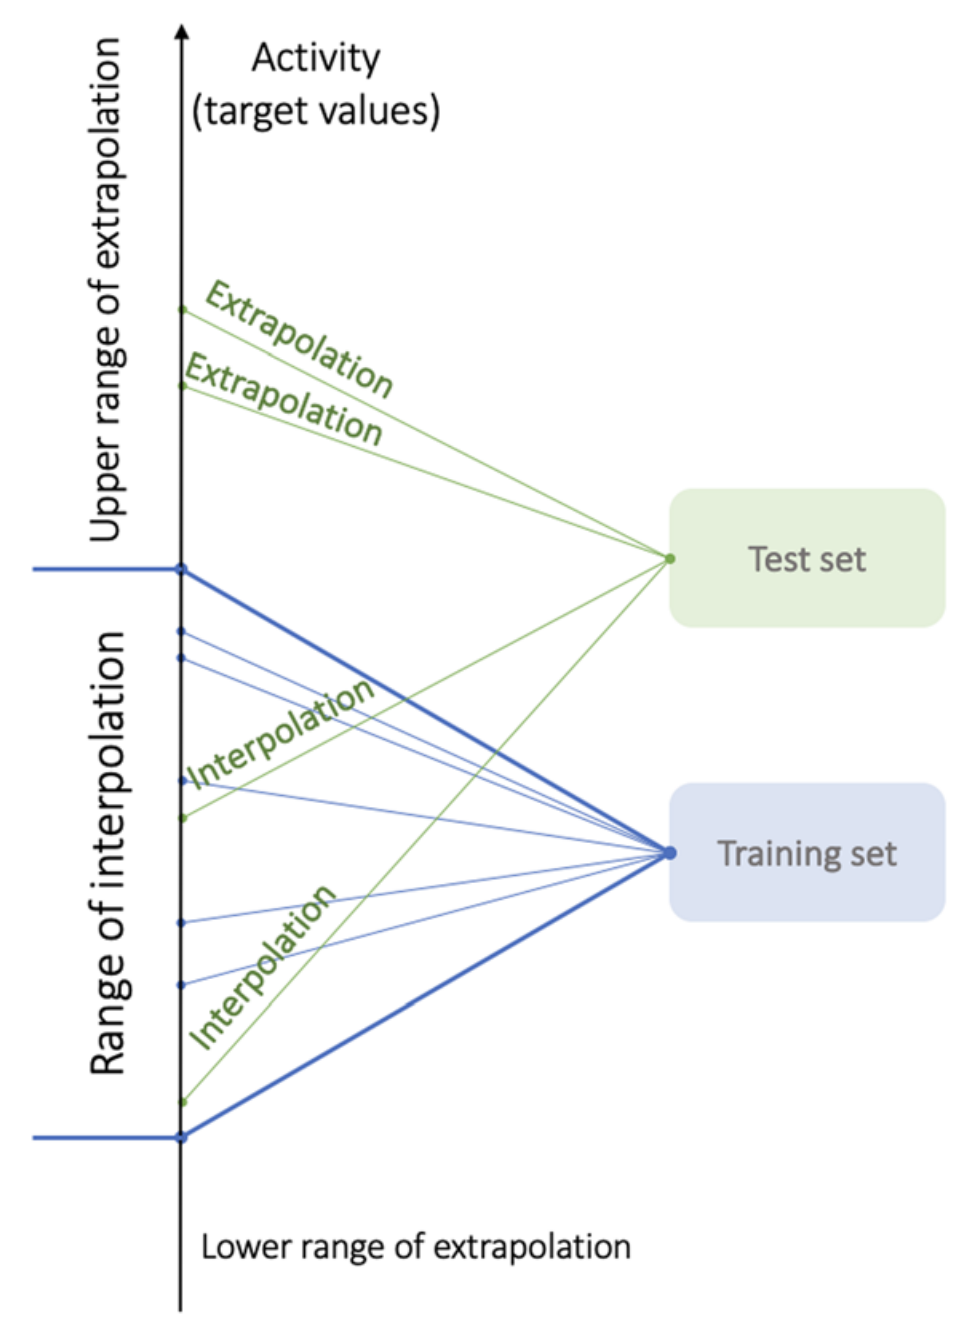
\includegraphics[width=\textwidth]{I-E.png}
        \end{figure}
    \end{minipage}
    \hfill
    \begin{minipage}[t]{0.52\textwidth}
        \vfill
        \begin{center}
            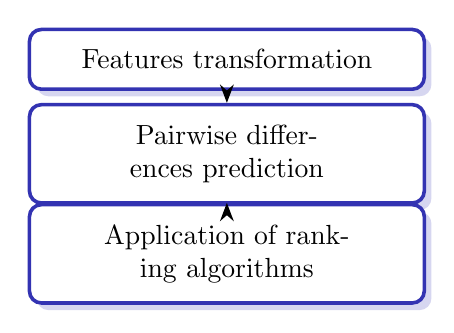
\begin{tikzpicture}[>={Stealth[scale=1]}, line width=0.15ex,
                every node/.style={
                        rectangle,
                        fill=white,
                        rounded corners=1ex,
                        line width=0.3ex,
                        text centered,
                        inner sep=1.7ex,
                        draw=blendedblue,
                        text width=4.5cm,
                        drop shadow={opacity=.2,fill=blendedblue,shadow xshift=0.6ex, shadow yshift=-0.6ex}}]

                \node (A) at (0, 1.2) {Features transformation};

                \node (B) at (0, 0) {Pairwise differences prediction};

                \node (C) at (0, -1.27) {Application of ranking algorithms};

                \draw[->, thick] (A) -- (B);
                \draw[->, thick] (B) -- (C);
            \end{tikzpicture}
        \end{center}
        \vfill
        \begin{block}{\small Key metrics}
            \footnotesize
            \begin{itemize}
                \item $f1_{top10}$ --- F1 score of a ML method to retrieve top 10\% samples.
                \item $f1_{extrap}$ --- F1 score of a ML method to retrieve extrapolating samples.
            \end{itemize}
        \end{block}
    \end{minipage}
\end{frame}

\end{document}
